\section{Online Learning with Hierarchical Experts}\label{sec:online}
In this section we look at an online decision making problem with structured/dependent experts. In online decision making, we have a finite number of experts $N$ and a finite number of rounds $T$. At each round we have to play an expert after which a loss value for each expert is revealed. The goal is to minimize the total loss incurred. There are many algorithms for this problem but the update time at each round depends linearly on $N$. In cases where the experts are structured (such as paths in a graph), under some structural assumptions on the losses, we can get much faster algorithms such as the ones presented in \cite{koolen2010hedging} and \cite{cortes2015line}. 

Motivated by hierachical classification studied in \cite{ramaswamy2015convex}, we look at experts arranged in a hierachical structure. For example, suppose every day one has to send one person from the Science school to attend a quiz. The exact topic of the quiz is unknown except for the fact that it will be a sub-field of Science. The experts are people with expertice in different branches of Science. Some have a broad knowledge of general topics such as Chemistry or Physics while some might have knowledge about very specific topics such as String Theory or Electrochemistry. In such cases the experts are naturally arranged in a tree. We formalize this as an online decision making problem with structure and provide a solution based on \cite{cortes2015line}.

\subsection{The Problem}
We have a complete rooted binary tree $\Tr$ of height $n$ with each node representing an expert. Given two nodes $y_1$ and $y_2$, let $d_\Tr(y_1,y_2)$ denote the tree distance between the two nodes, i.e., the length of the unique path from $y_1$ to $y_2$ in $\Tr$. The learning proceeds in rounds of interaction between the learner $\L$ and the environment as follows:\\

Learner $\L$: For $t = 1,...,T$,
\begin{itemize}
 \item Play expert $\hat{y}_t \in V(\Tr)$
 \item Receive best expert $y_t \in V(\Tr)$
 \item Incur loss $d_\Tr(\hat{y}_t,y_t)$
 \item Update model
\end{itemize}
We allow the learner to randomize the choice of $\hat{y}_t$ but the environment's choice of $y_t$ only depends on the probability distribution of $\hat{y}_t$ and not on the actual expert played. If we look at the quiz example, we can assume we have one expert for every topic and the true label gives the topic of the quiz on the particular day. Note that the tree need not be binary, but we assume binary trees for the sake of simplicity. 

Since there are only $N = 2^{n+1} - 1$ experts, we can associate a unique number to every expert in the range $[2^{n+1}-1]$ and hence each expert can be represented using only $O(n)$ bits. A more natural representation of each expert is using the location with respect to the root. The vertices of the binary tree $\Tr$ is taken to be $\{w \in \{0,1\}^* \mid |w| \leq n\}$ which is the set of binary sequences of length atmost $n$ and the parent of a node $w$ is obtained by removing the last bit from $w$. The root is repesented by the empty string $\epsilon$, $0$ is a child of $\epsilon$, $01$ is a child of $0$ and so on. The two representations are polynomial time inter-convertible as long as the numbering in the former representation is done in some natural way. We'll use the string/word based representation throughout the rest of this discussion.

The goal of a learning algorithm is twofold: (a) Play step and Update step runs in time polynomial in $n$ and does not depend on $N$. (b) For all sequences of true experts $y_1,...,y_T$, the regret is sub-linear in $T$, where the regret of a learner $\L$ is the total loss incurred minus the loss of the best expert in hindsight:
$$R(\L) = \sum_{t=1}^T d_\Tr(\hat{y}_t,y_t) - \min_{y \in V(\Tr)}\sum_{t=1}^T d_{\Tr}(y,y_t)$$

\textit{Non-linearity of the loss}: Note that the loss $d_\Tr$ is not linear in its first component with the string based representation of nodes. Nonetheless, can we represent each node $y$ as a vector $\u_y$ in $\{0,1\}^d$ and assign a loss vector $\lb_y \in \R_+^d$ to every node such that $d_\Tr(y_1,y_2) = \u_{y_1}^T\lb_{y_2}$? If we could, for small $d$, then we can apply the Component Hedge algorithm from \cite{koolen2010hedging}. But note that $d$ has to be atleast the rank of the $N$-by-$N$ matrix $M_\Tr$ given by $M_\Tr[y_1,y_2] = d_\Tr(y_1,y_2)$. We expect the rank of $M_\Tr$ to be high, although we are not aware of any known bounds.

\subsection{Background}
Our algorithm reduces this problem to the problem studied in Cortes et. al. 2015 \cite{cortes2015line} in which the authors study a class of problems in the online prediction with expert advice setting. In this setting, there is a prediction space $\Y$ and a finite number of experts. There is loss function $\ell:\Y\times\Y \to \R$. At each round $t$, a prediction/advice (in $\Y$) from each expert is revealed using which the learner predicts a $\hat{y}_t \in \Y$. Then the ``correct'' prediction $y_t$ is revealed and the learner incurs loss $\ell(\hat{y_t},y_t)$. 

To state the exact problem studied in the paper, we need some definitions. Let $\Sigma$ be a finite aphabet. Here, we set $\Sigma = \{0,1\}$. A finite automaton $A$ over $\Sigma$ is a tuple $(\Sigma,Q,I,F,E)$ where $Q$ is a finite set of states, $I\subseteq Q$ is the set of initial states, $F\subseteq Q$ is the set of final states and $E \subseteq Q \times (\Sigma \cup \epsilon) \times Q$ is a finite set of transitions (labeled edges) from state to state. We take the prediction space $\Y = \Sigma^*$. Every path from a state in $I$ to a state in $F$ is considered as an expert. At each round $t$, new labels on the edges are revealed. The advice of an expert $\xi$ at time $t$, denoted using $\xi(t)$, is the label of the path $\xi$ at time $t$.

The loss function $\ell: \Sigma^* \times \Sigma^* \to \R$ is given by a weighted finite state transducer WFST $\U$ over $\Sigma$. A WFST $\U$ is a tuple $(\Sigma,Q,I,F,E)$ where $Q$ is a finite set of states, $I \subseteq Q$ is the set of initial states, $F \subseteq Q$ is the set of final states and $E \subseteq Q \times (\Sigma\cup\epsilon)^2 \times \R_+ \times Q$ is a finite set of edges labeled by an input symbol, an output symbol and a weight. For any two strings $y_1,y_2 \in \Sigma^*$, let $P_\U(y_1,y_2)$ denote the set of paths from a state in $I$ to a state in $F$ with the input and output labels of the path being $y_1$ and $y_2$ respectively. The value of an input-output pair $(y_1,y_2) \in \Sigma^*\times\Sigma^*$ denoted by $\U(y_1,y_2)$ is the sum over all paths in $P_\U(y_1,y_2)$ the product of edge weights on the path.
$$\U(y_1,y_2) = \sum_{\pi \in P_\U(y_1,y_2)}\prod_{e\in\pi}\text{weight}(e)$$
where $\text{weight}((q_1,a_i,a_o,r,q_2)) = r$ and a path $\pi$ is viewed as a multiset of edges from $E$. $\U(y_1,y_2)$ is defined to be $0$ if $P_\U(y_1,y_2) = \emptyset$. The corresponding loss function $\ell_\U:\Sigma^*\times\Sigma^* \to \R$ is given by,
$$\ell_\U(y_1,y_2) = -\log(\U(y_1,y_2))$$
Finally, the online learning setting is as follows: There is a WFST $\U$ and a finite automaton $A$ whose (fixed) set of paths is the set of experts.

For rounds $t = 1,...,T$,
\begin{itemize}
 \item Receive new labels on edges of $A$
 \item Play $\hat{y}_t \in \Sigma^*$ based on predictions $\xi(t)$ of each expert $\xi$
 \item Receive correct prediction $y_t \in \Sigma^*$
 \item Incur loss $\ell_\U(\hat{y}_t,y_t)$
 \item Update model
\end{itemize}

The paper provides a Follow The Perturbed Leader (FTPL) based algorithm for this problem that runs in time polynomial in the size of $A$, $\U$ and $T$ if the underlying graphs are acyclic. The regret is also bounded by a constant.

\subsection{Reduction}

We can easily cast our hierarchical experts problem in the above language. Consider the following finite automaton $A$:
\begin{center}
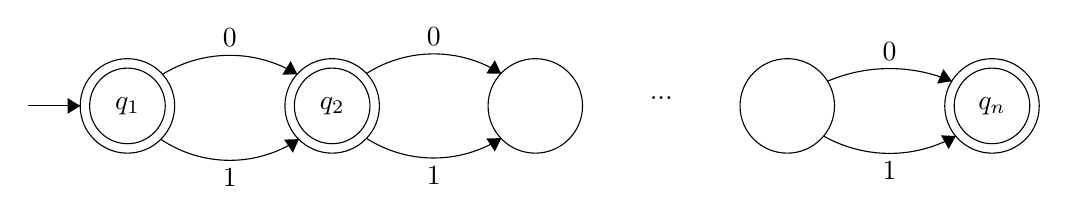
\begin{tikzpicture}[scale=0.2]
\tikzstyle{every node}+=[inner sep=0pt]
\draw [black] (8.8,-27.7) circle (3);
\draw (8.8,-27.7) node {$q_1$};
\draw [black] (8.8,-27.7) circle (2.4);
\draw [black] (21.8,-27.7) circle (3);
\draw (21.8,-27.7) node {$q_2$};
\draw [black] (21.8,-27.7) circle (2.4);
\draw [black] (34.7,-27.7) circle (3);
\draw [black] (50.7,-27.7) circle (3);
\draw [black] (63.7,-27.7) circle (3);
\draw (63.7,-27.7) node {$q_n$};
\draw [black] (63.7,-27.7) circle (2.4);
\draw [black] (11.013,-25.7) arc (121.60326:58.39674:8.18);
\fill [black] (19.59,-25.7) -- (19.17,-24.85) -- (18.64,-25.71);
\draw (15.3,-23.99) node [above] {$0$};
\draw [black] (19.693,-29.81) arc (-55.91527:-124.08473:7.839);
\fill [black] (19.69,-29.81) -- (18.75,-29.84) -- (19.31,-30.67);
\draw (15.3,-31.66) node [below] {$1$};
\draw [black] (23.966,-25.65) arc (122.61963:57.38037:7.948);
\fill [black] (32.53,-25.65) -- (32.13,-24.8) -- (31.59,-25.64);
\draw (28.25,-23.9) node [above] {$0$};
\draw [black] (32.536,-29.752) arc (-57.3416:-122.6584:7.943);
\fill [black] (32.54,-29.75) -- (31.59,-29.76) -- (32.13,-30.6);
\draw (28.25,-31.51) node [below] {$1$};
% \draw [black] (37.7,-27.7) -- (47.7,-27.7);
% \fill [black] (47.7,-27.7) -- (46.9,-27.2) -- (46.9,-28.2);
\draw (42.7,-27.2) node  {$...$};
\draw [black] (53.246,-26.135) arc (113.06476:66.93524:10.092);
\fill [black] (61.15,-26.13) -- (60.61,-25.36) -- (60.22,-26.28);
\draw (57.2,-24.83) node [above] {$0$};
\draw [black] (61.404,-29.606) arc (-60.40346:-119.59654:8.511);
\fill [black] (61.4,-29.61) -- (60.46,-29.57) -- (60.95,-30.44);
\draw (57.2,-31.22) node [below] {$1$};
\draw [black] (2.5,-27.7) -- (5.8,-27.7);
\fill [black] (5.8,-27.7) -- (5,-27.2) -- (5,-28.2);
\end{tikzpicture}
\end{center}
There are $n$ linearly arranged states with two transitions from one state to the next (one for each label 0 and 1). $q_1$ is the only initial state and every state is a final state. Hence, every path uniquely represents a node in the tree $\Tr$, specifically, the node represented by the label on the path. In our case, the advice of each expert/path remains the same for each round and is exacly the representation of the expert/node in $\Tr$. Now we need to represent the loss $d_{\Tr}$ using a WFST $\U$. Such a $\U$ is given below. The input and output labels on the edges are separated by a `$/$' and the weight is given in paranthesis.

\begin{center}
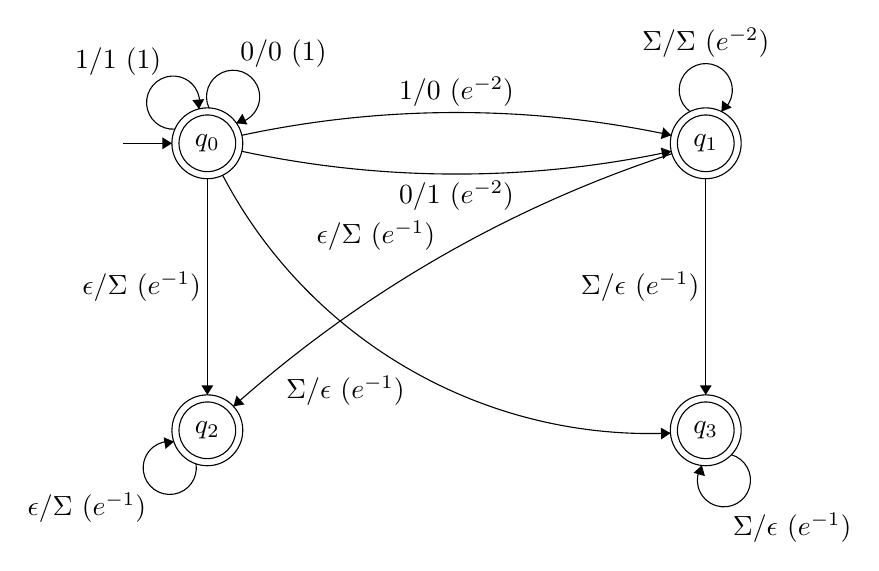
\begin{tikzpicture}[scale=0.15]
\tikzstyle{every node}+=[inner sep=0pt]
\draw [black] (19.8,-13.6) circle (3);
\draw (19.8,-13.6) node {$q_0$};
\draw [black] (19.8,-13.6) circle (2.4);
\draw [black] (62,-13.6) circle (3);
\draw (62,-13.6) node {$q_1$};
\draw [black] (62,-13.6) circle (2.4);
\draw [black] (19.8,-37.9) circle (3);
\draw (19.8,-37.9) node {$q_2$};
\draw [black] (19.8,-37.9) circle (2.4);
\draw [black] (62,-37.9) circle (3);
\draw (62,-37.9) node {$q_3$};
\draw [black] (62,-37.9) circle (2.4);
\draw [black] (12.7,-13.6) -- (16.8,-13.6);
\fill [black] (16.8,-13.6) -- (16,-13.1) -- (16,-14.1);
\draw [black] (19.941,-10.615) arc (205.03398:-82.96602:2.25);
\draw (26.25,-7.19) node [above] {$0/0\mbox{ }(1)$};
\fill [black] (22.25,-11.9) -- (23.19,-12.01) -- (22.77,-11.1);
\draw [black] (17.063,-12.4) arc (274.05479:-13.94521:2.25);
\draw (12.25,-7.94) node [above] {$1/1\mbox{ }(1)$};
\fill [black] (19.09,-10.7) -- (19.53,-9.86) -- (18.53,-9.94);
\draw [black] (22.722,-12.92) arc (102.10355:77.89645:86.695);
\fill [black] (59.08,-12.92) -- (58.4,-12.26) -- (58.19,-13.24);
\draw (40.9,-10.49) node [above] {$1/0\mbox{ }(e^{-2})$};
\draw [black] (59.078,-14.279) arc (-77.90311:-102.09689:86.742);
\fill [black] (59.08,-14.28) -- (58.19,-13.96) -- (58.4,-14.94);
\draw (40.9,-16.71) node [below] {$0/1\mbox{ }(e^{-2})$};
\draw [black] (60.677,-10.92) arc (234:-54:2.25);
\draw (62,-6.35) node [above] {$\Sigma/\Sigma\mbox{ }(e^{-2})$};
\fill [black] (63.32,-10.92) -- (64.2,-10.57) -- (63.39,-9.98);
\draw [black] (19.8,-16.6) -- (19.8,-34.9);
\fill [black] (19.8,-34.9) -- (20.3,-34.1) -- (19.3,-34.1);
\draw (19.3,-25.75) node [left] {$\epsilon/\Sigma\mbox{ }(e^{-1})$};
\draw [black] (22.008,-35.869) arc (131.79304:108.07616:104.244);
\fill [black] (22.01,-35.87) -- (22.94,-35.71) -- (22.27,-34.96);
\draw (34.07,-22.74) node [above] {$\epsilon/\Sigma\mbox{ }(e^{-1})$};
\draw [black] (18.84,-40.73) arc (9:-279:2.25);
\draw (9.6,-43.15) node [below] {$\epsilon/\Sigma\mbox{ }(e^{-1})$};
\fill [black] (16.97,-38.86) -- (16.1,-38.49) -- (16.26,-39.48);
\draw [black] (62,-16.6) -- (62,-34.9);
\fill [black] (62,-34.9) -- (62.5,-34.1) -- (61.5,-34.1);
\draw (61.5,-25.75) node [left] {$\Sigma/\epsilon\mbox{ }(e^{-1})$};
\draw [black] (59.01,-38.138) arc (-87.55222:-152.31699:40.846);
\fill [black] (59.01,-38.14) -- (58.19,-37.67) -- (58.23,-38.67);
\draw (31.49,-33.23) node [below] {$\Sigma/\epsilon\mbox{ }(e^{-1})$};
\draw [black] (64.159,-39.966) arc (73.98311:-214.01689:2.25);
\draw (69.31,-44.89) node [below] {$\Sigma/\epsilon\mbox{ }(e^{-1})$};
\fill [black] (61.67,-40.87) -- (60.97,-41.5) -- (61.93,-41.78);
\end{tikzpicture}
\end{center}

$q_0$ is the only initial state and every state is a final state. The underlying automaton of $\U$  automaton is determiistic and $P_\U(y_1,y_2)$ is a singleton for every pair of experts $y_1$ and $y_2$. The transducer ignores the longest common prefix and multiplies $e^{-2}$ as long as both strings still have symbols to be read and then multiplies $e^{-1}$ for the rest of the remaining string. It is easy to see that for any two experts/nodes in $\Tr$, $y_1$ and $y_2$, $\U(y_1,y_2) = \exp(-d_{\Tr}(y_1,y_2))$ giving us that $\ell_{\U}(y_1,y_2) = d_{\Tr}(y_1,y_2)$. Note that $\U$ is not acyclic but can be made acyclic by making $n$ copies and adding transitions from one copy to another.

Hence if we use the solution from \cite{cortes2015line} with the automaton $A$ (same label for every time step) and loss given by $\U$, we get a solution running in time polynomial in $|A|$, $|\U|$ and $T$ and hence polynomial in $n$ and $T$. The regret bound we get is,
$$\E[R(\L)] \leq 8n\sqrt{N(1+2\log(n))L_{min}} + 64n^2N(1+2\log(n))$$
The expectation is under the randomness of the algorithm and $L_{min}$ is the cumulative loss of the best expert in hindsight. 

\subsection{Further Work}
Although the runtime is polynomial in $n$ and does not depend on $N$, the solution uses an FTPL style algorithm causing the memory used and time taken in round $t$ to be linear in $t$ which is not feasible in most cases. Also, the regret bound, inspite of being sublinear in $T$, depends on $N$ which is large. One possible direction is to design a new online learning algorithm directly for the hierarchical experts case that does not have such limitations.